%!TEX TS-program = xelatex

% Шаблон документа LaTeX создан в 2018 году
% Алексеем Подчезерцевым
% В качестве исходных использованы шаблоны
% 	Данилом Фёдоровых (danil@fedorovykh.ru) 
%		https://www.writelatex.com/coursera/latex/5.2.2
%	LaTeX-шаблон для русской кандидатской диссертации и её автореферата.
%		https://github.com/AndreyAkinshin/Russian-Phd-LaTeX-Dissertation-Template

\documentclass[a4paper,14pt]{article}


%%% Работа с русским языком
\usepackage[english,russian]{babel}   %% загружает пакет многоязыковой вёрстки
\usepackage{fontspec}      %% подготавливает загрузку шрифтов Open Type, True Type и др.
\defaultfontfeatures{Ligatures={TeX},Renderer=Basic}  %% свойства шрифтов по умолчанию
\setmainfont[Ligatures={TeX,Historic}]{Times New Roman} %% задаёт основной шрифт документа
\setsansfont{Comic Sans MS}                    %% задаёт шрифт без засечек
\setmonofont{Courier New}
\usepackage{indentfirst}
\frenchspacing

\renewcommand{\epsilon}{\ensuremath{\varepsilon}}
\renewcommand{\phi}{\ensuremath{\varphi}}
\renewcommand{\kappa}{\ensuremath{\varkappa}}
\renewcommand{\le}{\ensuremath{\leqslant}}
\renewcommand{\leq}{\ensuremath{\leqslant}}
\renewcommand{\ge}{\ensuremath{\geqslant}}
\renewcommand{\geq}{\ensuremath{\geqslant}}
\renewcommand{\emptyset}{\varnothing}

%%% Дополнительная работа с математикой
\usepackage{amsmath,amsfonts,amssymb,amsthm,mathtools} % AMS
\usepackage{icomma} % "Умная" запятая: $0,2$ --- число, $0, 2$ --- перечисление

%% Номера формул
%\mathtoolsset{showonlyrefs=true} % Показывать номера только у тех формул, на которые есть \eqref{} в тексте.
%\usepackage{leqno} % Нумерация формул слева	

%% Перенос знаков в формулах (по Львовскому)
\newcommand*{\hm}[1]{#1\nobreak\discretionary{}
	{\hbox{$\mathsurround=0pt #1$}}{}}

%%% Работа с картинками
\usepackage{graphicx}  % Для вставки рисунков
\graphicspath{{images/}}  % папки с картинками
\setlength\fboxsep{3pt} % Отступ рамки \fbox{} от рисунка
\setlength\fboxrule{1pt} % Толщина линий рамки \fbox{}
\usepackage{wrapfig} % Обтекание рисунков текстом

%%% Работа с таблицами
\usepackage{array,tabularx,tabulary,booktabs} % Дополнительная работа с таблицами
\usepackage{longtable}  % Длинные таблицы
\usepackage{multirow} % Слияние строк в таблице
\usepackage{float}% http://ctan.org/pkg/float

%%% Программирование
\usepackage{etoolbox} % логические операторы


%%% Страница
\usepackage{extsizes} % Возможность сделать 14-й шрифт
\usepackage{geometry} % Простой способ задавать поля
\geometry{top=20mm}
\geometry{bottom=20mm}
\geometry{left=20mm}
\geometry{right=10mm}
%
%\usepackage{fancyhdr} % Колонтитулы
% 	\pagestyle{fancy}
%\renewcommand{\headrulewidth}{0pt}  % Толщина линейки, отчеркивающей верхний колонтитул
% 	\lfoot{Нижний левый}
% 	\rfoot{Нижний правый}
% 	\rhead{Верхний правый}
% 	\chead{Верхний в центре}
% 	\lhead{Верхний левый}
%	\cfoot{Нижний в центре} % По умолчанию здесь номер страницы

\usepackage{setspace} % Интерлиньяж
\onehalfspacing % Интерлиньяж 1.5
%\doublespacing % Интерлиньяж 2
%\singlespacing % Интерлиньяж 1

\usepackage{lastpage} % Узнать, сколько всего страниц в документе.

\usepackage{soul} % Модификаторы начертания

\usepackage{hyperref}
\usepackage[usenames,dvipsnames,svgnames,table,rgb]{xcolor}
\hypersetup{				% Гиперссылки
	unicode=true,           % русские буквы в раздела PDF
	pdftitle={Заголовок},   % Заголовок
	pdfauthor={Автор},      % Автор
	pdfsubject={Тема},      % Тема
	pdfcreator={Создатель}, % Создатель
	pdfproducer={Производитель}, % Производитель
	pdfkeywords={keyword1} {key2} {key3}, % Ключевые слова
	colorlinks=true,       	% false: ссылки в рамках; true: цветные ссылки
	linkcolor=black,          % внутренние ссылки
	citecolor=black,        % на библиографию
	filecolor=magenta,      % на файлы
	urlcolor=black           % на URL
}
\makeatletter 
\def\@biblabel#1{#1. } 
\makeatother
\usepackage{cite} % Работа с библиографией
%\usepackage[superscript]{cite} % Ссылки в верхних индексах
%\usepackage[nocompress]{cite} % 
\usepackage{csquotes} % Еще инструменты для ссылок

\usepackage{multicol} % Несколько колонок

\usepackage{tikz} % Работа с графикой
\usepackage{pgfplots}
\usepackage{pgfplotstable}

% ГОСТ заголовки
\usepackage[font=small]{caption}
%\captionsetup[table]{justification=centering, labelsep = newline} % Таблицы по правобу краю
%\captionsetup[figure]{justification=centering} % Картинки по центру


\newcommand{\tablecaption}[1]{\addtocounter{table}{1}\small \begin{flushright}\tablename \ \thetable\end{flushright}%	
\begin{center}#1\end{center}}

\newcommand{\imref}[1]{рис.~\ref{#1}}

\usepackage{multirow}
\usepackage{spreadtab}
\newcolumntype{K}[1]{@{}>{\centering\arraybackslash}p{#1cm}@{}}


\usepackage{xparse}
\ExplSyntaxOn
\DeclareExpandableDocumentCommand{\juliandate}{ m m m }
{
	\juliandate_calc:nnnn { #1 } { #2 } { #3 } { \use:n }
}
\NewDocumentCommand{\storejuliandate}{ s m m m m }
{
	\IfBooleanTF{#1}
	{
		\juliandate_calc:nnnn { #3 } { #4 } { #5 } { \cs_set:Npx #2 }
	}
	{
		\juliandate_calc:nnnn { #3 } { #4 } { #5 } { \cs_new:Npx #2 }
	}
}
\cs_new:Npn \juliandate_calc:nnnn #1 #2 #3 #4 % #1 = day, #2 = month, #3 = year, #4 = what to do
{
	#4 
	{
		\int_eval:n
		{
			#1 +
			\int_div_truncate:nn { 153 * (#2 + 12 * \int_div_truncate:nn { 14 - #2 } { 12 } - 3) + 2 } { 5 } +
			365 * (#3 + 4800 - \int_div_truncate:nn { 14 - #2 } { 12 } ) +
			\int_div_truncate:nn { #3 + 4800 - \int_div_truncate:nn { 14 - #2 } { 12 } } { 4 } -
			\int_div_truncate:nn { #3 + 4800 - \int_div_truncate:nn { 14 - #2 } { 12 } } { 100 } + 
			\int_div_truncate:nn { #3 + 4800 - \int_div_truncate:nn { 14 - #2 } { 12 } } { 400 } -
			32045
		}
	}
}

\tl_new:N \l__juliandate_g_tl
\tl_new:N \l__juliandate_dg_tl
\tl_new:N \l__juliandate_c_tl
\tl_new:N \l__juliandate_dc_tl
\tl_new:N \l__juliandate_b_tl
\tl_new:N \l__juliandate_db_tl
\tl_new:N \l__juliandate_a_tl
\tl_new:N \l__juliandate_da_tl
\tl_new:N \l__juliandate_y_tl
\tl_new:N \l__juliandate_m_tl
\tl_new:N \l__juliandate_d_tl
\int_new:N \l_juliandate_day_int
\int_new:N \l_juliandate_month_int
\int_new:N \l_juliandate_year_int

\cs_new:Npn \__juliandate_set:nn #1 #2
{
	\tl_set:cx { l__juliandate_#1_tl } { \int_eval:n { #2 } }
}
\cs_new:Npn \__juliandate_use:n #1
{
	\tl_use:c { l__juliandate_#1_tl }
}
\cs_new_protected:Npn \juliandate_reverse:n #1
{
	\__juliandate_set:nn { g }
	{ \int_div_truncate:nn { #1 + 32044 } { 146097 } }
	\__juliandate_set:nn { dg }
	{ \int_mod:nn { #1 + 32044 } { 146097 } }
	\__juliandate_set:nn { c }
	{ \int_div_truncate:nn { ( \int_div_truncate:nn { \__juliandate_use:n { dg } } { 36524 } + 1) * 3 } { 4 } }
	\__juliandate_set:nn { dc }
	{ \__juliandate_use:n { dg } - \__juliandate_use:n { c } * 36524 }
	\__juliandate_set:nn { b }
	{ \int_div_truncate:nn { \__juliandate_use:n { dc } } { 1461 } }
	\__juliandate_set:nn { db }
	{ \int_mod:nn { \__juliandate_use:n { dc } } { 1461 } }
	\__juliandate_set:nn { a }
	{ \int_div_truncate:nn { ( \int_div_truncate:nn { \__juliandate_use:n { db } } { 365 } + 1) * 3 } { 4 } }
	\__juliandate_set:nn { da }
	{ \__juliandate_use:n { db } - \__juliandate_use:n { a } * 365 }
	\__juliandate_set:nn { y }
	{
		\__juliandate_use:n { g } * 400 + 
		\__juliandate_use:n { c } * 100 + 
		\__juliandate_use:n { b } * 4 + 
		\__juliandate_use:n { a }
	}
	\__juliandate_set:nn { m }
	{ \int_div_truncate:nn { \__juliandate_use:n { da } * 5 + 308 } { 153 } - 2 }
	\__juliandate_set:nn { d }
	{ \__juliandate_use:n { da } - \int_div_truncate:nn { (\__juliandate_use:n { m } + 4) * 153 } { 5 } + 122 }
	\int_set:Nn \l_juliandate_year_int
	{ \__juliandate_use:n { y } - 4800 + \int_div_truncate:nn { \__juliandate_use:n { m } + 2 } { 12 } }
	\int_set:Nn \l_juliandate_month_int
	{ \int_mod:nn { \__juliandate_use:n { m } + 2 } { 12 } + 1 }
	\int_set:Nn \l_juliandate_day_int
	{ \__juliandate_use:n { d } + 1 }
}
\cs_generate_variant:Nn \juliandate_reverse:n { x }

\NewDocumentCommand{\showday}{ m }
{
	\juliandate_reverse:n { #1 }
	\int_to_arabic:n { \l_juliandate_day_int }-
	\int_to_arabic:n { \l_juliandate_month_int }-
	\int_to_arabic:n { \l_juliandate_year_int }
}

\NewDocumentCommand{\tomorrow}{ }
{
	\group_begin:
	\juliandate_reverse:x { \juliandate_calc:nnnn { \day + 1 } { \month } { \year } { \use:n } }
	\day = \l_juliandate_day_int
	\month = \l_juliandate_month_int
	\year = \l_juliandate_year_int
	\today
	\group_end:
}
\NewDocumentCommand{\tomorrowof}{ m m m }
{
	\group_begin:
	\juliandate_reverse:x { \juliandate_calc:nnnn { #1 + 1 } { #2 } { #3 } { \use:n } }
	\day = \l_juliandate_day_int
	\month = \l_juliandate_month_int
	\year = \l_juliandate_year_int
	\today
	\group_end:
}
\ExplSyntaxOff
\begin{document} % конец преамбулы, начало документа
\begin{titlepage}
	\begin{center}
		ФЕДЕРАЛЬНОЕ  ГОСУДАРСТВЕННОЕ АВТОНОМНОЕ \\
		ОБРАЗОВАТЕЛЬНОЕ УЧРЕЖДЕНИЕ ВЫСШЕГО ОБРАЗОВАНИЯ\\
		«НАЦИОНАЛЬНЫЙ ИССЛЕДОВАТЕЛЬСКИЙ УНИВЕРСИТЕТ\\
		«ВЫСШАЯ ШКОЛА ЭКОНОМИКИ»
	\end{center}
	
	\begin{center}
		\textbf{Московский институт электроники и математики}
		
		\textbf{Им. А.Н.Тихонова НИУ ВШЭ}
		
		\textbf{Департамент электронной инженерии}
	\end{center}
	\vspace{1ex}	
	\begin{center}
		Подчезерцев Алексей Евгеньевич, группа БИВ172
		
		Солодянкин Андрей Александрович, группа БИВ172
	\end{center}	
	\vspace{1ex}
	\begin{center}
		\textbf{ОТЧЕТ\\
		ПО ЛАБОРАТОРНОЙ РАБОТЕ №2
	}
	\end{center}	
	\vspace{2ex}
	\begin{center}
		по дисциплине «Схемотехника»
	\end{center}
	\vspace{2ex}
	\begin{center}
	Дата сдачи отчета: \today
	\end{center}
	\vspace{2ex}
	\vfill
	\begin{center}
		Москва \the\year г.
	\end{center}
\end{titlepage}
%\tableofcontents
\pagebreak
\section{Исходные и рассчитанные параметры}

Выбор и подсчет исходных значений:
\begin{itemize}

\item Тип фильтра: Баттерворта ($\alpha = 1.414; \varepsilon = 1.000$)

\item $f_{cp} = 2kHz$

\item Выбор R

$R_1 = R_2 = R_a = R = 10 k\Omega$

\item Определение C

$f_{cp} = \dfrac{1}{2\pi RC}$

$C = \dfrac{1}{2\pi Rf_{cp}} = \dfrac{1}{2\pi * 10k\Omega * 2kHz}$

$C_1 = C_2 = C = 7.958 nF$

\item $R_b = (2-\alpha)R_a = (2 - 1.414)10k\Omega = 5860 \Omega$

\item $Ku_{teor} = \dfrac{U_{out}}{U_{in}} = \dfrac{I_{OC}(R_b + R_a)}{I_{OC}R_a} = \dfrac{R_b}{R_a} + 1 = \dfrac{(2 - \alpha) R_a}{R_a} + 1 = 3 - \alpha = 1.586$
\end{itemize}

\section{Фильтр низких частот}

\subsection{Построение схемы}

Схема фильтра нижних частот представлена на рис. \ref{fig:shfnch}.

\begin{figure}[H]
	\centering
	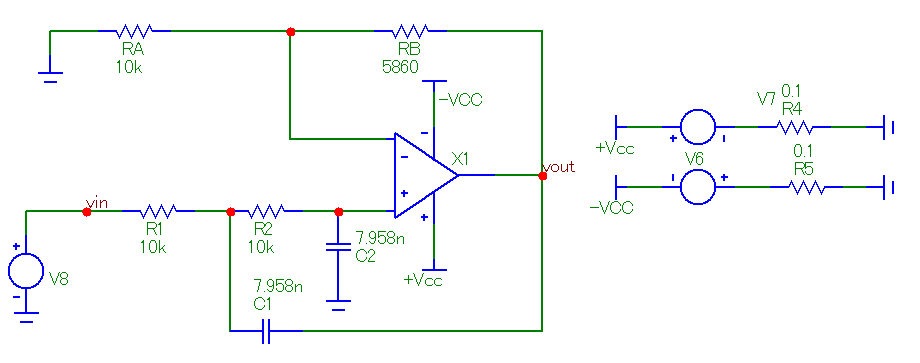
\includegraphics[width=0.85\linewidth]{../imgs/FNCH/sh_fnch}
	\caption{Схема фильтра низких частот}
	\label{fig:shfnch}
\end{figure}

\subsection{Получение АЧХ и ФЧХ}

Построим графики АЧХ и ФЧХ (рис. \ref{fig:afchn}).

\begin{figure}[H]
	\centering
	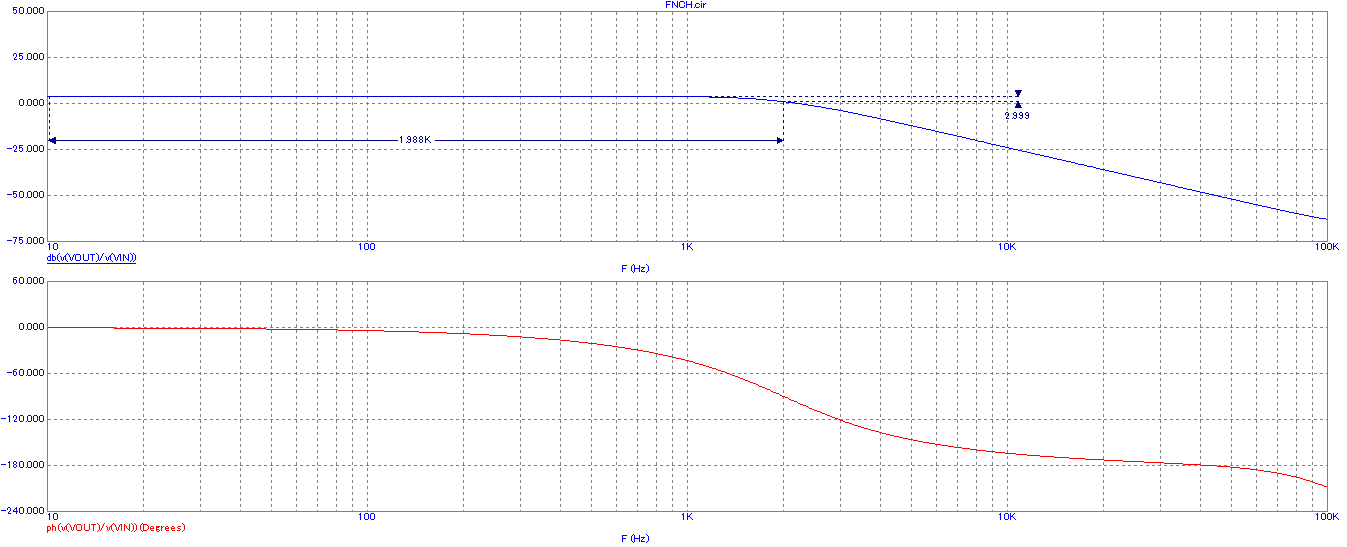
\includegraphics[width=0.85\linewidth]{../imgs/FNCH/AFcH_N}
	\caption{АЧХ и ФЧХ с измерением частоты среза}
	\label{fig:afchn}
\end{figure}

Фактическая частота среза получилась $1.999kHz \approx 2kHz$.

Полоса пропускания находится в интервале $(0;2)kHz$.

\subsection{Получение динамических характеристик}

Построим график динамической характеристики для частот $500Hz$ (рис. \ref{fig:garm500n}) и $50kHz$ (рис. \ref{fig:garm50kn}).

\begin{figure}[H]
	\centering
	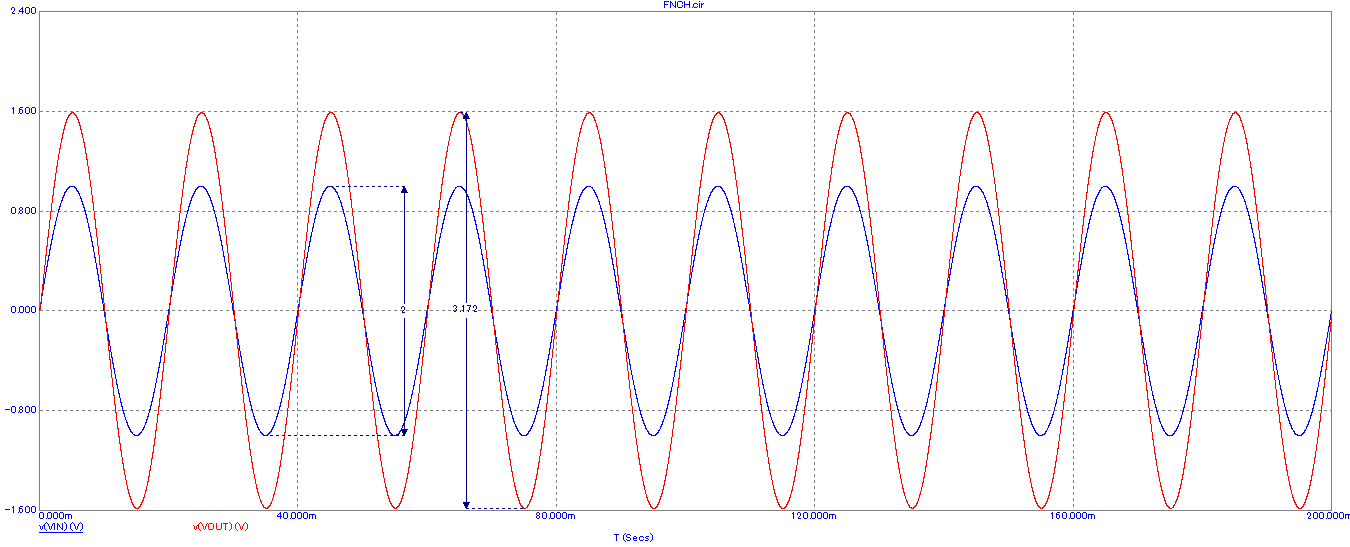
\includegraphics[width=0.95\linewidth]{../imgs/FNCH/garm_500_N}
	\caption{Динамическая характеристика ФНЧ для частоты $500Hz$}
	\label{fig:garm500n}
\end{figure}

Размах напряжения входного сигнала $2V$

Размах напряжения выходного сигнала $3.172V$

Рассчитаем фактический коэффициент усиления:

$Ku_{fact} = \dfrac{3.172V}{2V} = 1.586$

$Ku_{teor} = 1.586$

$Ku_{teor} = Ku_{fact}$

Коэффициент передачи 

\begin{figure}[H]
	\centering
	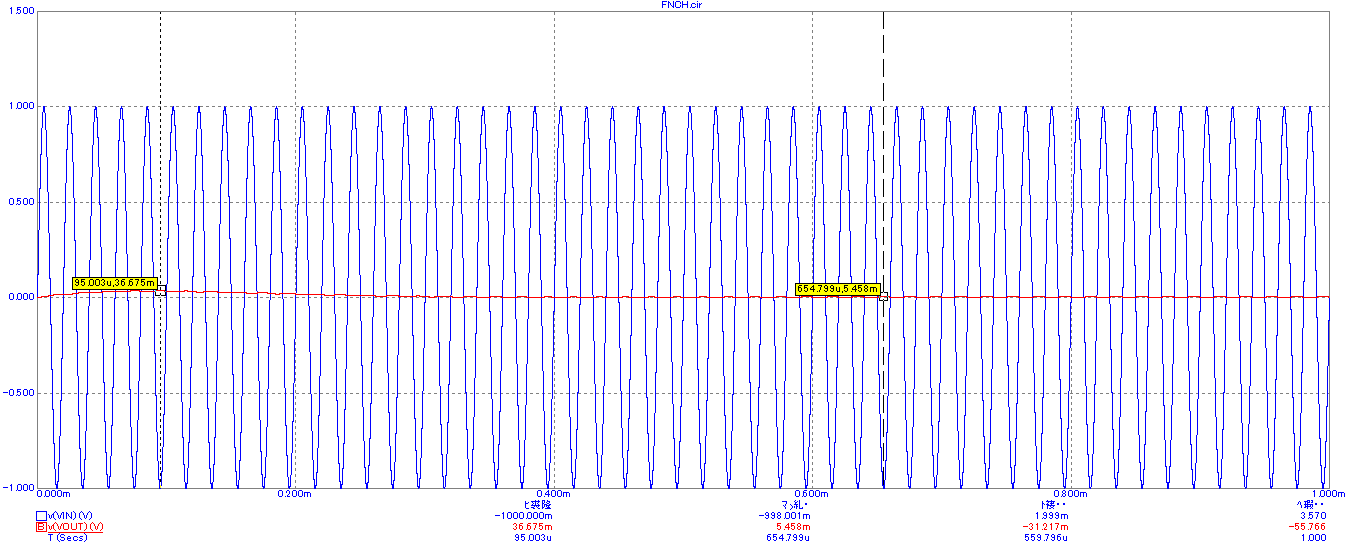
\includegraphics[width=0.95\linewidth]{../imgs/FNCH/garm_50k_N}
	\caption{Динамическая характеристика ФНЧ для частоты $50kHz$}
	\label{fig:garm50kn}
\end{figure}

Напряжение на повторяющихся локальных максимумах $U_{out} \approx 5.5mV$

$Ku = \dfrac{5.5mV}{1V} = 0.0055$

Выходное напряжение пренебрежимо мало по отношению ко входному, из этого можно сделать вывод, что сигнал данной частоты не пропускается через данный фильтр.

\subsection{Исследование влияния погрешностей}

Найдем зависимость между частотой среза и погрешностью сопротивления (рис. \ref{fig:pogrrn}). 

$R_{pogr} = 0.9R$

\begin{figure}[H]
	\centering
	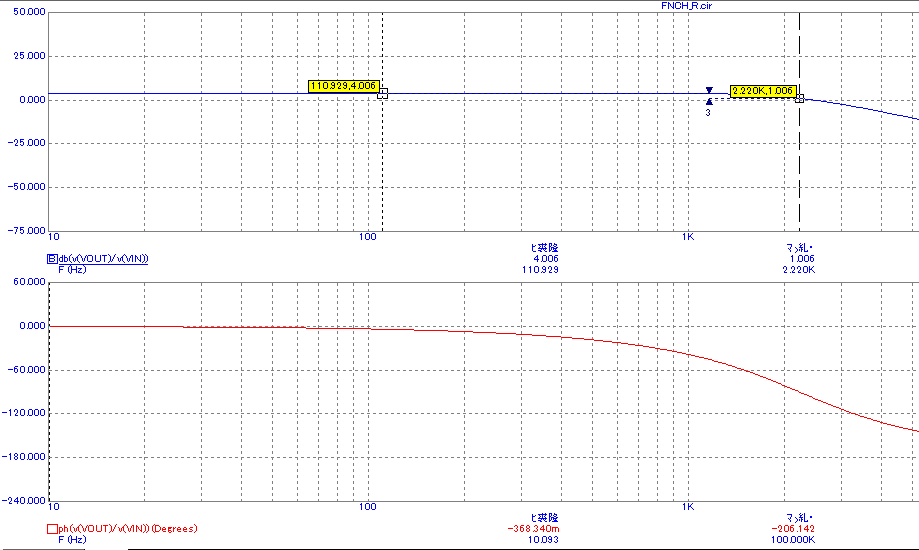
\includegraphics[width=0.85\linewidth]{../imgs/FNCH/pogr_R_N}
	\caption{АЧХ и ФЧХ для ФНЧ с уменьшенным сопротивлением}
	\label{fig:pogrrn}
\end{figure}

В данном случае частота среза стала больше, и составляет $2.22KHz$.

Найдем зависимость между частотой среза и погрешностью емкости (рис. \ref{fig:pogrcn}). 

$C_{pogr} = 0.9C$

\begin{figure}[H]
	\centering
	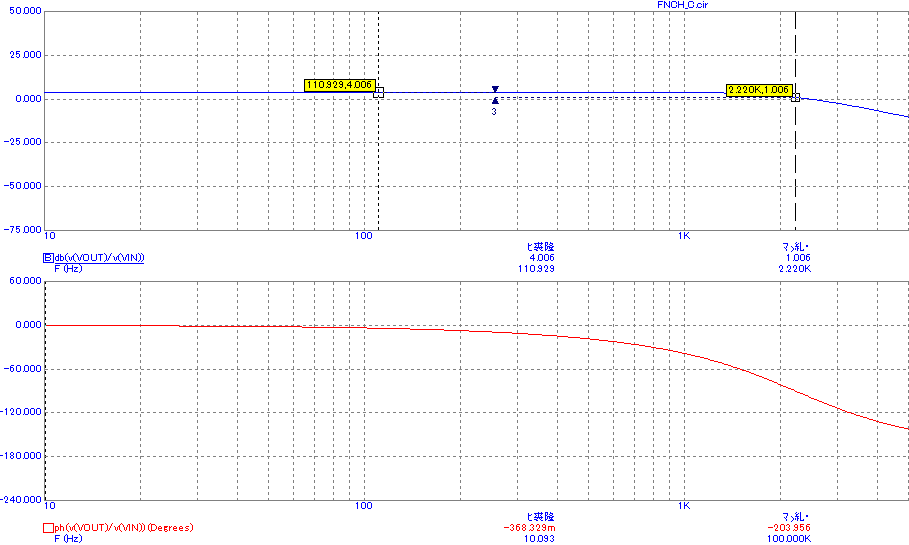
\includegraphics[width=0.85\linewidth]{../imgs/FNCH/pogr_C_N}
	\caption{АЧХ и ФЧХ для ФНЧ с уменьшенной емкостью}
	\label{fig:pogrcn}
\end{figure}

В данном случае частота среза стала больше, и также составляет $2.22KHz$.

Из проделанных опытов можно сделать вывод, что уменьшение сопротивления или емкости увеличивает частоту среза.

Действительно, частота среза обратно зависит $R$ и $C$ и находится по формуле:

$f_{cp} = \dfrac{1}{2\pi RC}$

Можно заметить, что при изменении $R$ и $C$ в одно и то же число раз, получена одна и та же частота среза.
Это можно также объяснить формулой, по которой находится частота среза.

\section{Фильтр высоких частот}

\subsection{Построение схемы}

Схема фильтра высоких частот представлена на рис. \ref{fig:shfvch}.


\begin{figure}[H]
	\centering
	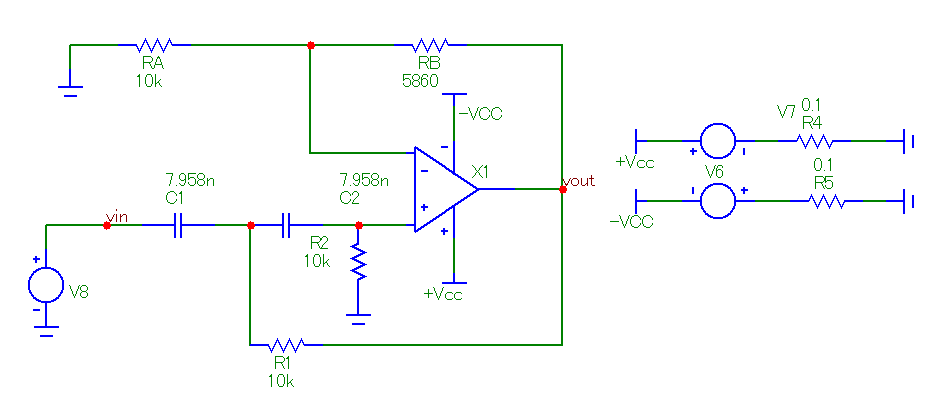
\includegraphics[width=0.85\linewidth]{../imgs/FVCH/sh_fvch}
	\caption{Схема фильтра высоких частот}
	\label{fig:shfvch}
\end{figure}


\subsection{Получение АЧХ и ФЧХ}

Построим графики АЧХ и ФЧХ (рис. \ref{fig:afchv1}).

\begin{figure}[H]
	\centering
	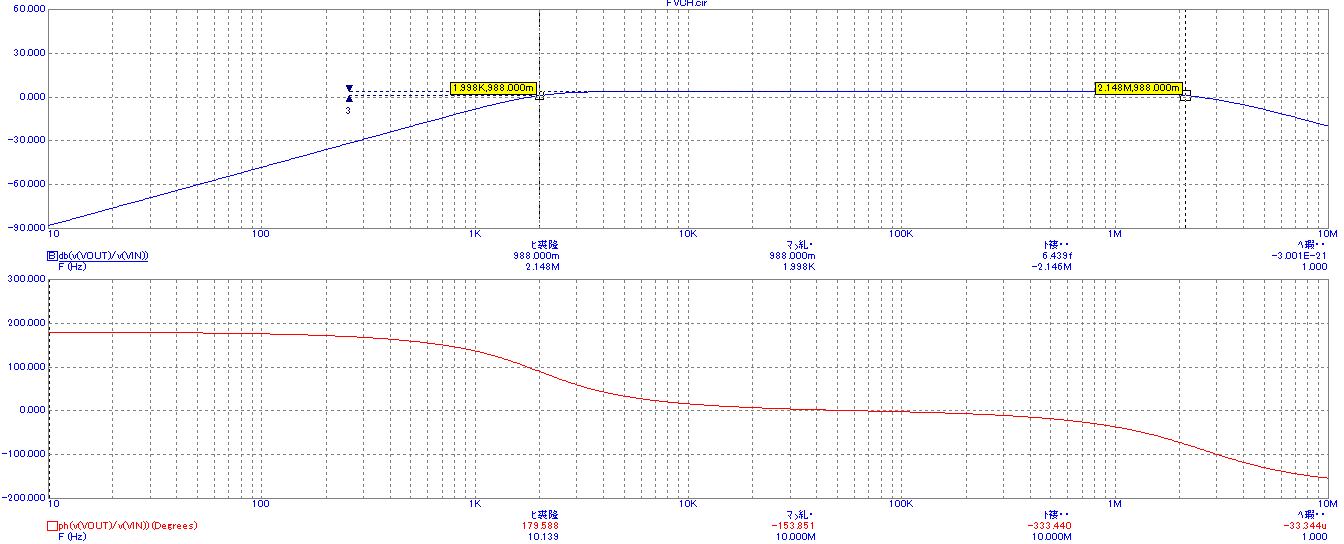
\includegraphics[width=0.85\linewidth]{../imgs/FVCH/AFcH_V1}
	\caption{АЧХ и ФЧХ с измерением частоты среза}
	\label{fig:afchv1}
\end{figure}


Фактическая частота среза получилась $1.998kHz \approx 2kHz$.

Полоса пропускания находится в интервале $(2kHz; 2.148MHz)$.


\subsection{Получение динамических характеристик}

Построим график динамической характеристики для частот $50Hz$ (рис. \ref{fig:garm50v}) и $50kHz$ (рис. \ref{fig:garm50kv}).

\begin{figure}[H]
	\centering
	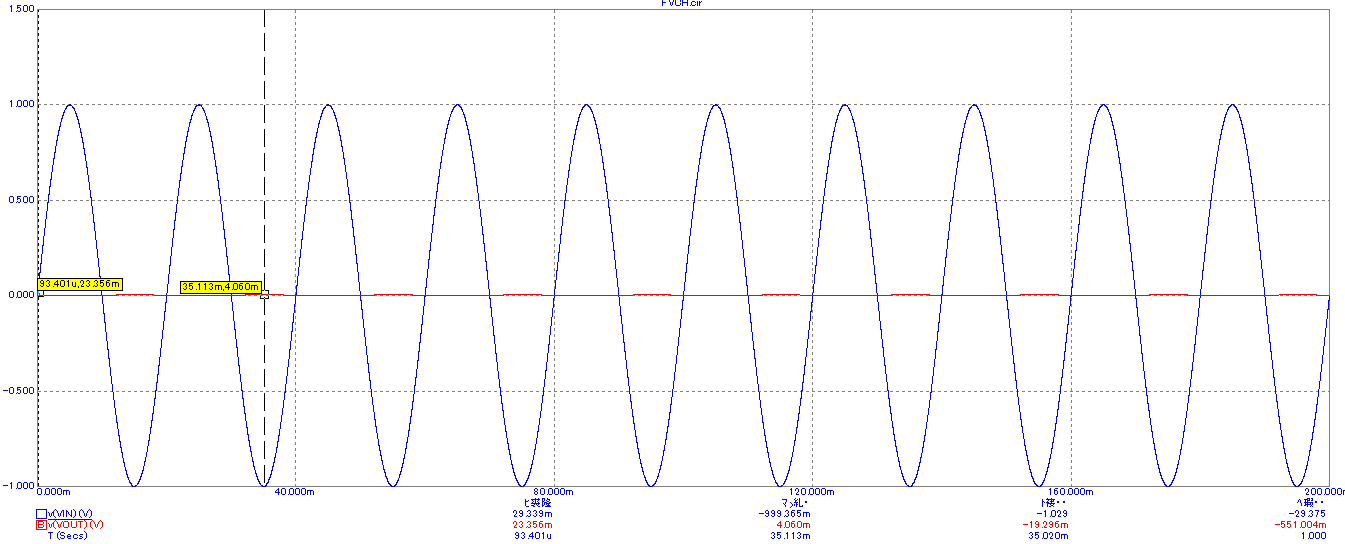
\includegraphics[width=0.95\linewidth]{../imgs/FVCH/garm_50_V}
	\caption{Динамическая характеристика ФВЧ для частоты $50Hz$}
	\label{fig:garm50v}
\end{figure}


Напряжение на повторяющихся локальных максимумах $U_{out} \approx 4mV$

$Ku = \dfrac{4mV}{1V} = 0.004$

Выходное напряжение пренебрежимо мало по отношению ко входному, из этого можно сделать вывод, что сигнал данной частоты не пропускается через данный фильтр.


\begin{figure}[H]
	\centering
	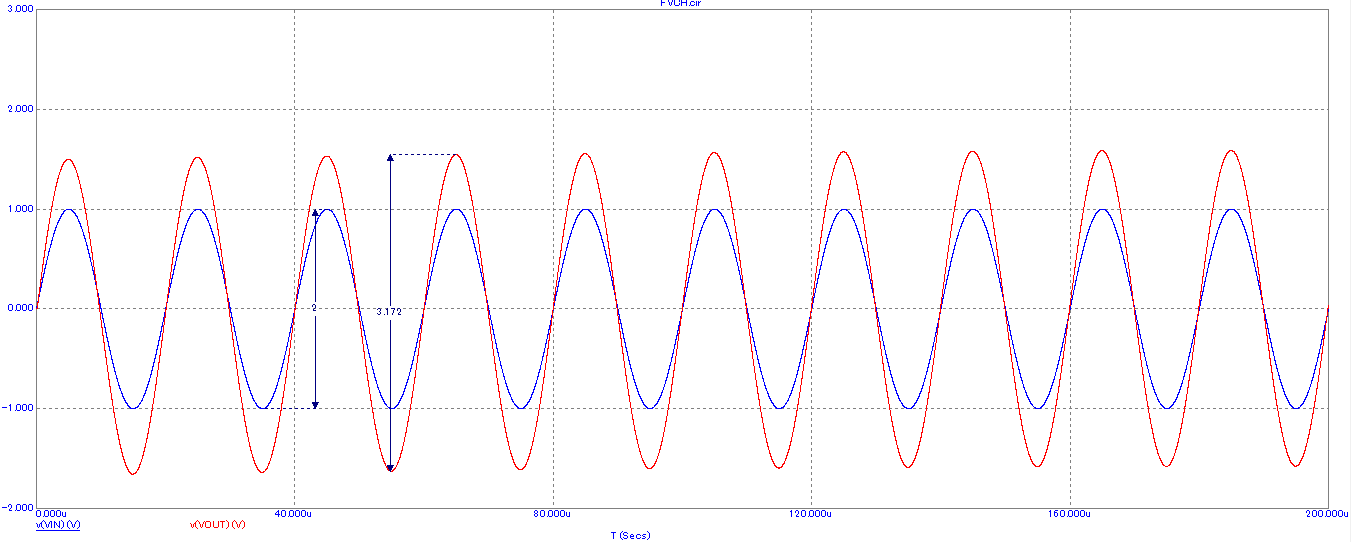
\includegraphics[width=0.95\linewidth]{../imgs/FVCH/garm_50k_V}
	\caption{Динамическая характеристика ФВЧ для частоты $50kHz$}
	\label{fig:garm50kv}
\end{figure}

Размах напряжения входного сигнала $2V$

Размах напряжения выходного сигнала $3.172V$

Рассчитаем фактический коэффициент усиления:

$Ku_{fact} = \dfrac{3.172V}{2V} = 1.586$

$Ku_{teor} = 1.586$

$Ku_{teor} = Ku_{fact}$


\subsection{Исследование влияния погрешностей}

Найдем зависимость между частотой среза и погрешностью сопротивления (рис. \ref{fig:pogrrv}). 

$R_{pogr} = 1.1R$

\begin{figure}[H]
	\centering
	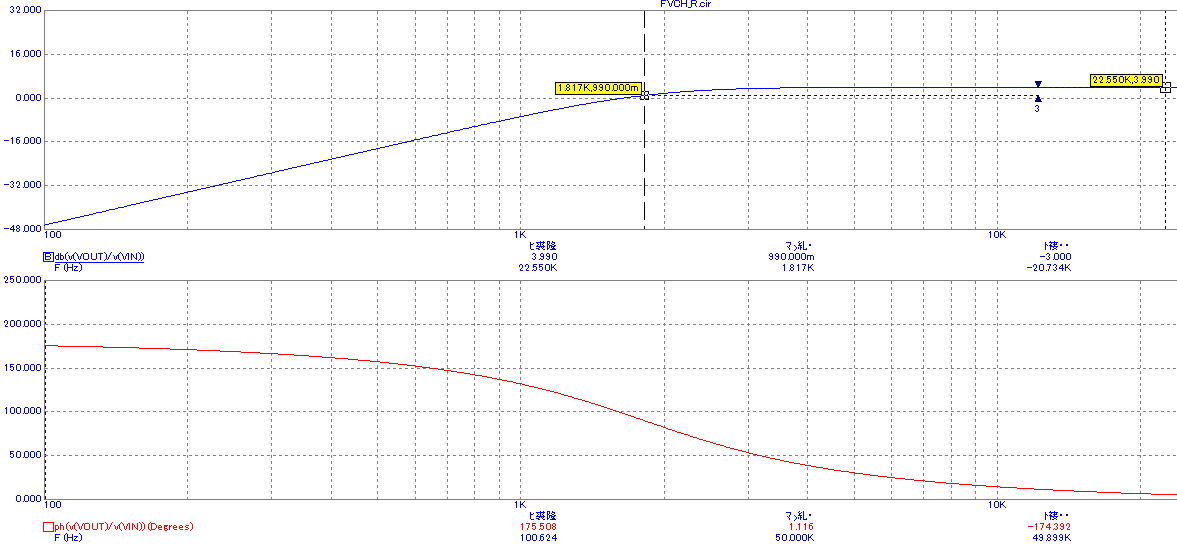
\includegraphics[width=0.85\linewidth]{../imgs/FVCH/pogr_R_V}
	\caption{АЧХ и ФЧХ для ФВЧ с увеличенным сопротивлением}
	\label{fig:pogrrv}
\end{figure}

В данном случае частота среза стала меньше, и составляет $1.817KHz$.

Найдем зависимость между частотой среза и погрешностью емкости (рис. \ref{fig:pogrcv}). 

$C_{pogr} = 1.1C$

\begin{figure}[H]
	\centering
	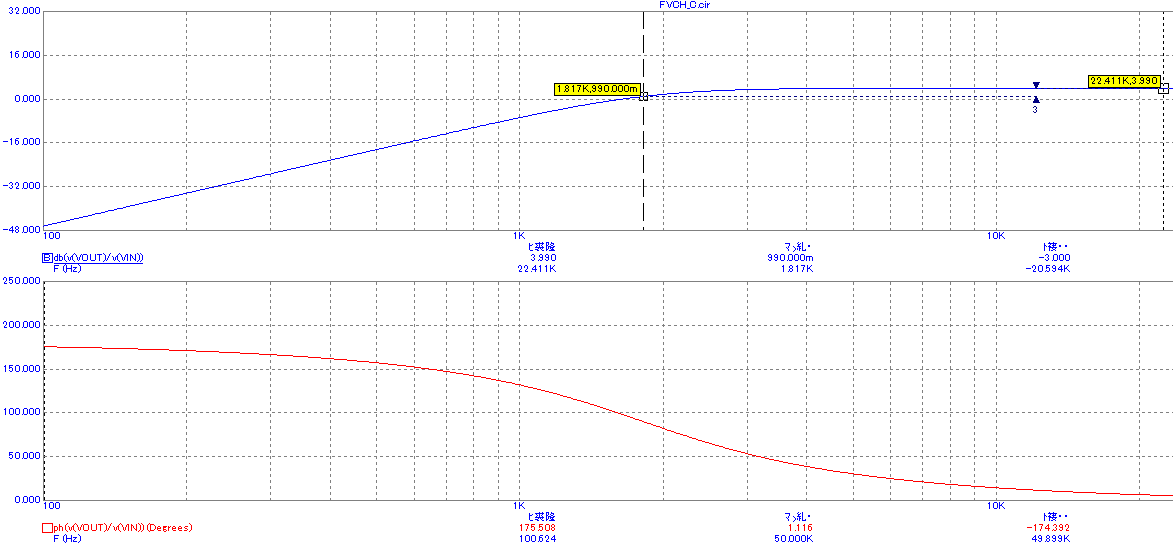
\includegraphics[width=0.85\linewidth]{../imgs/FVCH/pogr_C_V}
	\caption{АЧХ и ФЧХ для ФВЧ с увеличенной емкостью}
	\label{fig:pogrcv}
\end{figure}

В данном случае частота среза стала меньше, и также составляет $1.817KHz$.

Из проделанных опытов можно сделать вывод, что увеличение сопротивления или емкости уменьшает частоту среза.

Действительно, частота среза обратно зависит $R$ и $C$ и находится по формуле:

$f_{cp} = \dfrac{1}{2\pi RC}$

Можно заметить, что при изменении $R$ и $C$ в одно и то же число раз, получена одна и та же частота среза.
Это можно также объяснить формулой, по которой находится частота среза.

\section{Подгон параметров}

Изменим схемы следующим образом:

\begin{figure}[H]
	\centering
	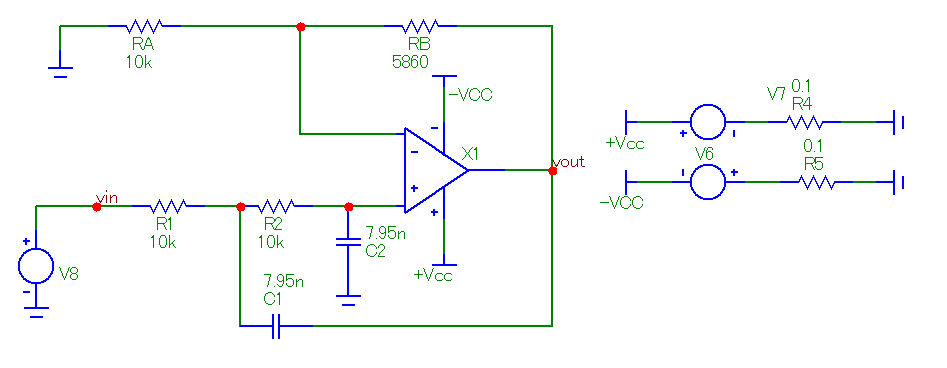
\includegraphics[width=0.85\linewidth]{../imgs/FNCH/sh_fnch_p}
	\caption{ФНЧ с подогнанными параметрами}
	\label{fig:shfnchp}
\end{figure}


\begin{figure}[H]
	\centering
	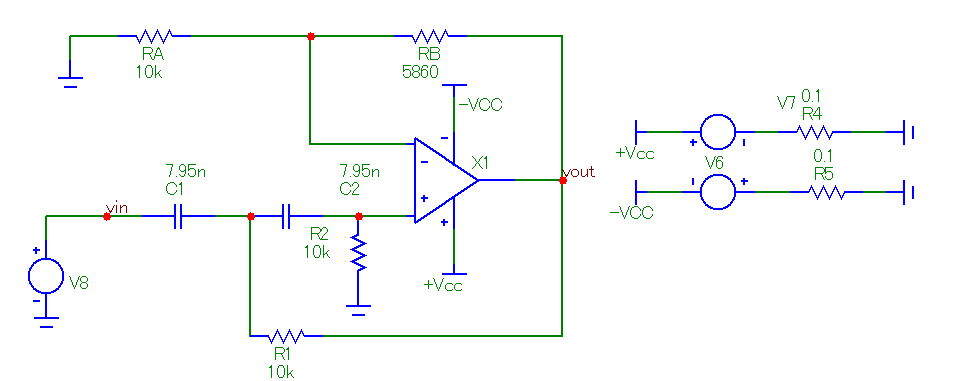
\includegraphics[width=0.85\linewidth]{../imgs/FVCH/sh_fvch_p}
	\caption{ФВЧ с подогнанными параметрами}
	\label{fig:shfvchp}
\end{figure}

Полученные АЧХ и ФЧХ для ФНЧ и ФВЧ:

\begin{figure}[H]
	\centering
	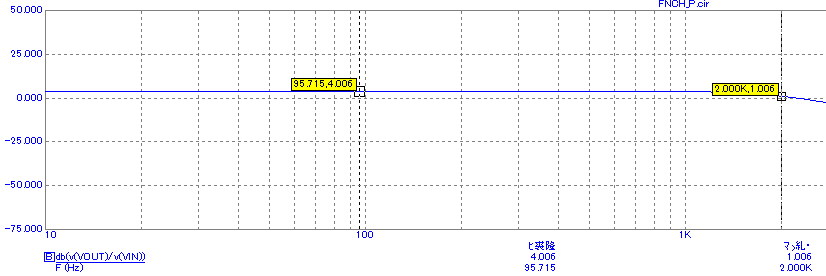
\includegraphics[width=0.85\linewidth]{../imgs/FNCH/gr_fnch_p1}
	\caption{АЧХ и ФЧХ для ФНЧ}
	\label{fig:grfnchp1}
\end{figure}


\begin{figure}[H]
	\centering
	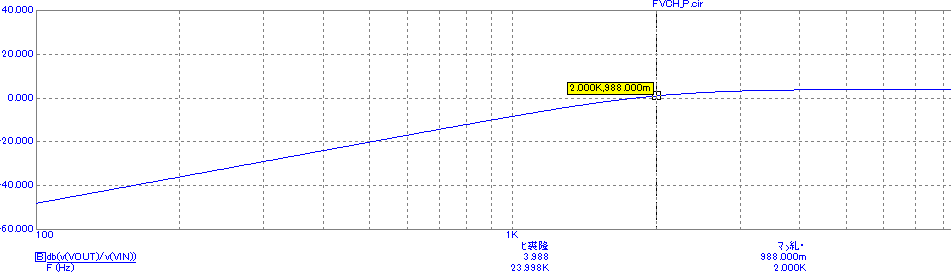
\includegraphics[width=0.85\linewidth]{../imgs/FVCH/gr_fvch_p1}
	\caption{АЧХ и ФЧХ для ФВЧ}
	\label{fig:grfvchp1}
\end{figure}

$Ku_{teor}$ идеально совпадает с $Ku_{pract}$ для ФНЧ и ФВЧ и без подгона.

\end{document} % конец документа






